\begin{table}[!t]
\centering
\caption{Simulation parameters}
\label{tab:sim-params}
\resizebox{\linewidth}{!}{%
\footnotesize
\begin{tabular}{llcc}
\hline
\textbf{Simulation parameter}       & \multicolumn{3}{c}{\textbf{Values}}                                         \\ \hline
Simulation time                     & \multicolumn{3}{l}{\unit[1.5]{h}}                                           \\
\# Nodes                            & \multicolumn{3}{l}{1 center root, 100 nodes in grid}                        \\
Mobility Model                      & \multicolumn{3}{l}{CRWP}                                                    \\
Application data packets            & \multicolumn{3}{l}{\unitfrac[20]{pkt}{node}, Rate = \unitfrac[1]{pkt}{min}} \\
Radio environment                   & \multicolumn{3}{l}{\unit[50]{m} UDGM constant loss}                         \\
Area of deployment                  & \multicolumn{3}{l}{\unit[400]{m} $\times$\unit[400]{m}}                     \\
Reverse Trickle                     & \multicolumn{3}{l}{$I_{max} = $ \unit[60]{s}, $I_{min} = $ \unit[1]{s}, $I_k = 3$}  \\
RPL Trickle                         & \multicolumn{3}{l}{$I_{max} = $ \unit[60]{s}}                               \\
\texttt{keepRoute} beaconing period & \multicolumn{3}{l}{$\delta = $ \unit[60]{s}}                         \\
$Mtable$                            & \multicolumn{3}{l}{$TTL_{max} = $ \unit[90]{s}, Size = \unit[20]{entries}}  \\
RPL downwards table                 & \multicolumn{3}{l}{Size = \unit[20]{entries}}                               \\
\# mobility traces                  & \multicolumn{3}{l}{\unitfrac[10]{traces}{scenario}}                         \\
Number of experiments               & \multicolumn{3}{l}{\unitfrac[10]{runs}{trace}}                              \\
Node Speed                          & \multicolumn{3}{l}{constant \unitfrac[4]{m}{s}}                             \\
$T_{pause}$                         & \multicolumn{3}{l}{constant \unit[300]{s}}                                  \\
\# node stops                       & \multicolumn{3}{l}{Uniform Dist. in $[1, 3]$ stops}                         \\ %\hline
%\multicolumn{4}{c}{\textbf{Mobility Scenarios}}                                                                   \\ %\hline
                                    & \multicolumn{1}{c}{\textbf{Low}}    & \textbf{Moderate}   & \textbf{High}   \\
PerMobNode                          & \multicolumn{1}{c}{$5\%$}           & $10\%$              & $15\%$          \\ \hline
\end{tabular}
}
\end{table}

\section{Simulation Results}
\label{sec:evaluation}

We implement $\mu$Matrix as a subroutine of collection protocol available in ContikiOS~\cite{dunkels:2004} and the experiments were run on Cooja~\cite{eriksson:2009}. We compare $\mu$Matrix with ContikiOS' RPL implementation. We use the BonnMotion~\cite{aschenbruck2010bonnmotion} to implement CRWP as well as to generate and analyze mobility traces. We simulated four different scenarios. The first scenario represents the static network, in which nodes do not move. The remaining represent mobility scenarios named low, moderate, and high with mobile nodes. Table~\ref{tab:sim-params} lists the default simulation parameters used for each scenario. 

On top of the network layer, we ran an application, in which each node sends $20$ data packets to the root. Upon receiving a data packet, the root confirms to the sender with an ack packet that has the size of a data packet. The application waits for \unit[10]{min} for protocols initialization and stabilization before it starts sending data. The nodes start sending their data in a simulation time randomly chosen in $(10, 20]$ min. The mobility traces were configured to start after the stabilization time. Additionally, we generate $10$ mobility traces for each scenario. Each trace and the static scenario were run $10$ times, totaling $3010$ runs. In each plot, the bars represent the average, and the error bars the confidence interval of \unit[95]{\%}, and the curves are the maximum table usage for a given mobility scenario.

\begin{table}[!ht]
\centering
\caption{Mobility Metrics}
\label{tab:mob}
\resizebox{\linewidth}{!}{%
\begin{tabular}{@{}lccc@{}}
\toprule
\multicolumn{1}{c}{Mobility Metrics} & Low Mob. sce. & Mod. Mob. sce. & High Mob. sce. \\ \midrule
Avg. Link Breaks                     & 1621          & 3057           & 4838           \\
Avg. Link duration                   & 761.90        & 457.4          & 345            \\
Avg. Degree                          & 4.12          & 4.36           & 4.44           \\
Avg. Time to link break              & 227.6         & 216.1          & 204.5          \\
\bottomrule
\end{tabular}
}
\end{table}

\noindent \textbf{Mobility scenario:} We simulated a scenario, where $n=100$ people are assumed to be in an office and can move around and return to a predefined home position. This scenario is expected to present relatively low mobility, thus in our set up, \unit[$k$]{\%} of the nodes are moving at any moment in time, where $k \in \{5, 10, 15\}$. Table~\ref{tab:mob} presents some mobility metrics~\cite{aschenbruck2010bonnmotion} for each scenario. We highlight that link breaks play a key role in the performance of the network protocol, note that high mobility scenario presents up to \unit[20]{\%} more topology changes than in low mobility. As expected, the average link duration decrease when $PerMobNode$ increases. The averages of node degrees and the time to a link break do not show much variability, they reflect the simulation parameters, where the node deployment is a grid and time for a link to break is less than $T_{pause}$. 

\subsection{Results}

In Figure~\ref{fig:memory-usage}, we show the Cumulative Distribution Functions (CDFs) of the percentage of downward routing table usage among nodes for given mobility scenario. In static scenarios, all $\mu$Matrix nodes use up to $25\%$ of available downwards route entries, while RPL $< 75\%$ of nodes use up to $25\%$ of entries. Indeed, for some RPL nodes, $100\%$ of table entries are used. Usually, those nodes that use more memory are near to the root, and they play a fundamental role in top-down routing. If they have a full downward routing table, then the traffic pattern top-down suffers from poor reliability, and some nodes may be unreachable. In mobility scenarios, $\mu$Matrix also presents more efficient memory footprint, and the difference grows up in high mobility scenarios, where $>50\%$ of RPL nodes have all table entries busy, while $\mu$Matrix nodes use at most $70\%$ of downwards available routes.

Figure~\ref{fig:beacons} shows the amount of control traffic overhead of the protocols (the total number of beacons sent during the entire simulation). RPL sends fewer control packets than $\mu$Matrix, but the difference between them does not exceed $7.4\%$. $\mu$Matrix sends more beacons to react to topology changes quickly. Reverse Trickle is responsible for firing most of $\mu$Matrix beacons. $\mu$Matrix allows tuning the Reverse Trickle fire rate to reduce the sending beacons, but note that the adjustment reverse trickle faces a  trade-off between quick mobility discovery and control overhead. In Table~\ref{tab:sim-params}, we set $I_{max}$ of RPL and $\mu$Matrix evenly and close to data packet rate, which gives to the protocols the fair opportunity to identify topology changes and react to them.

\begin{figure}[!t]
\centering
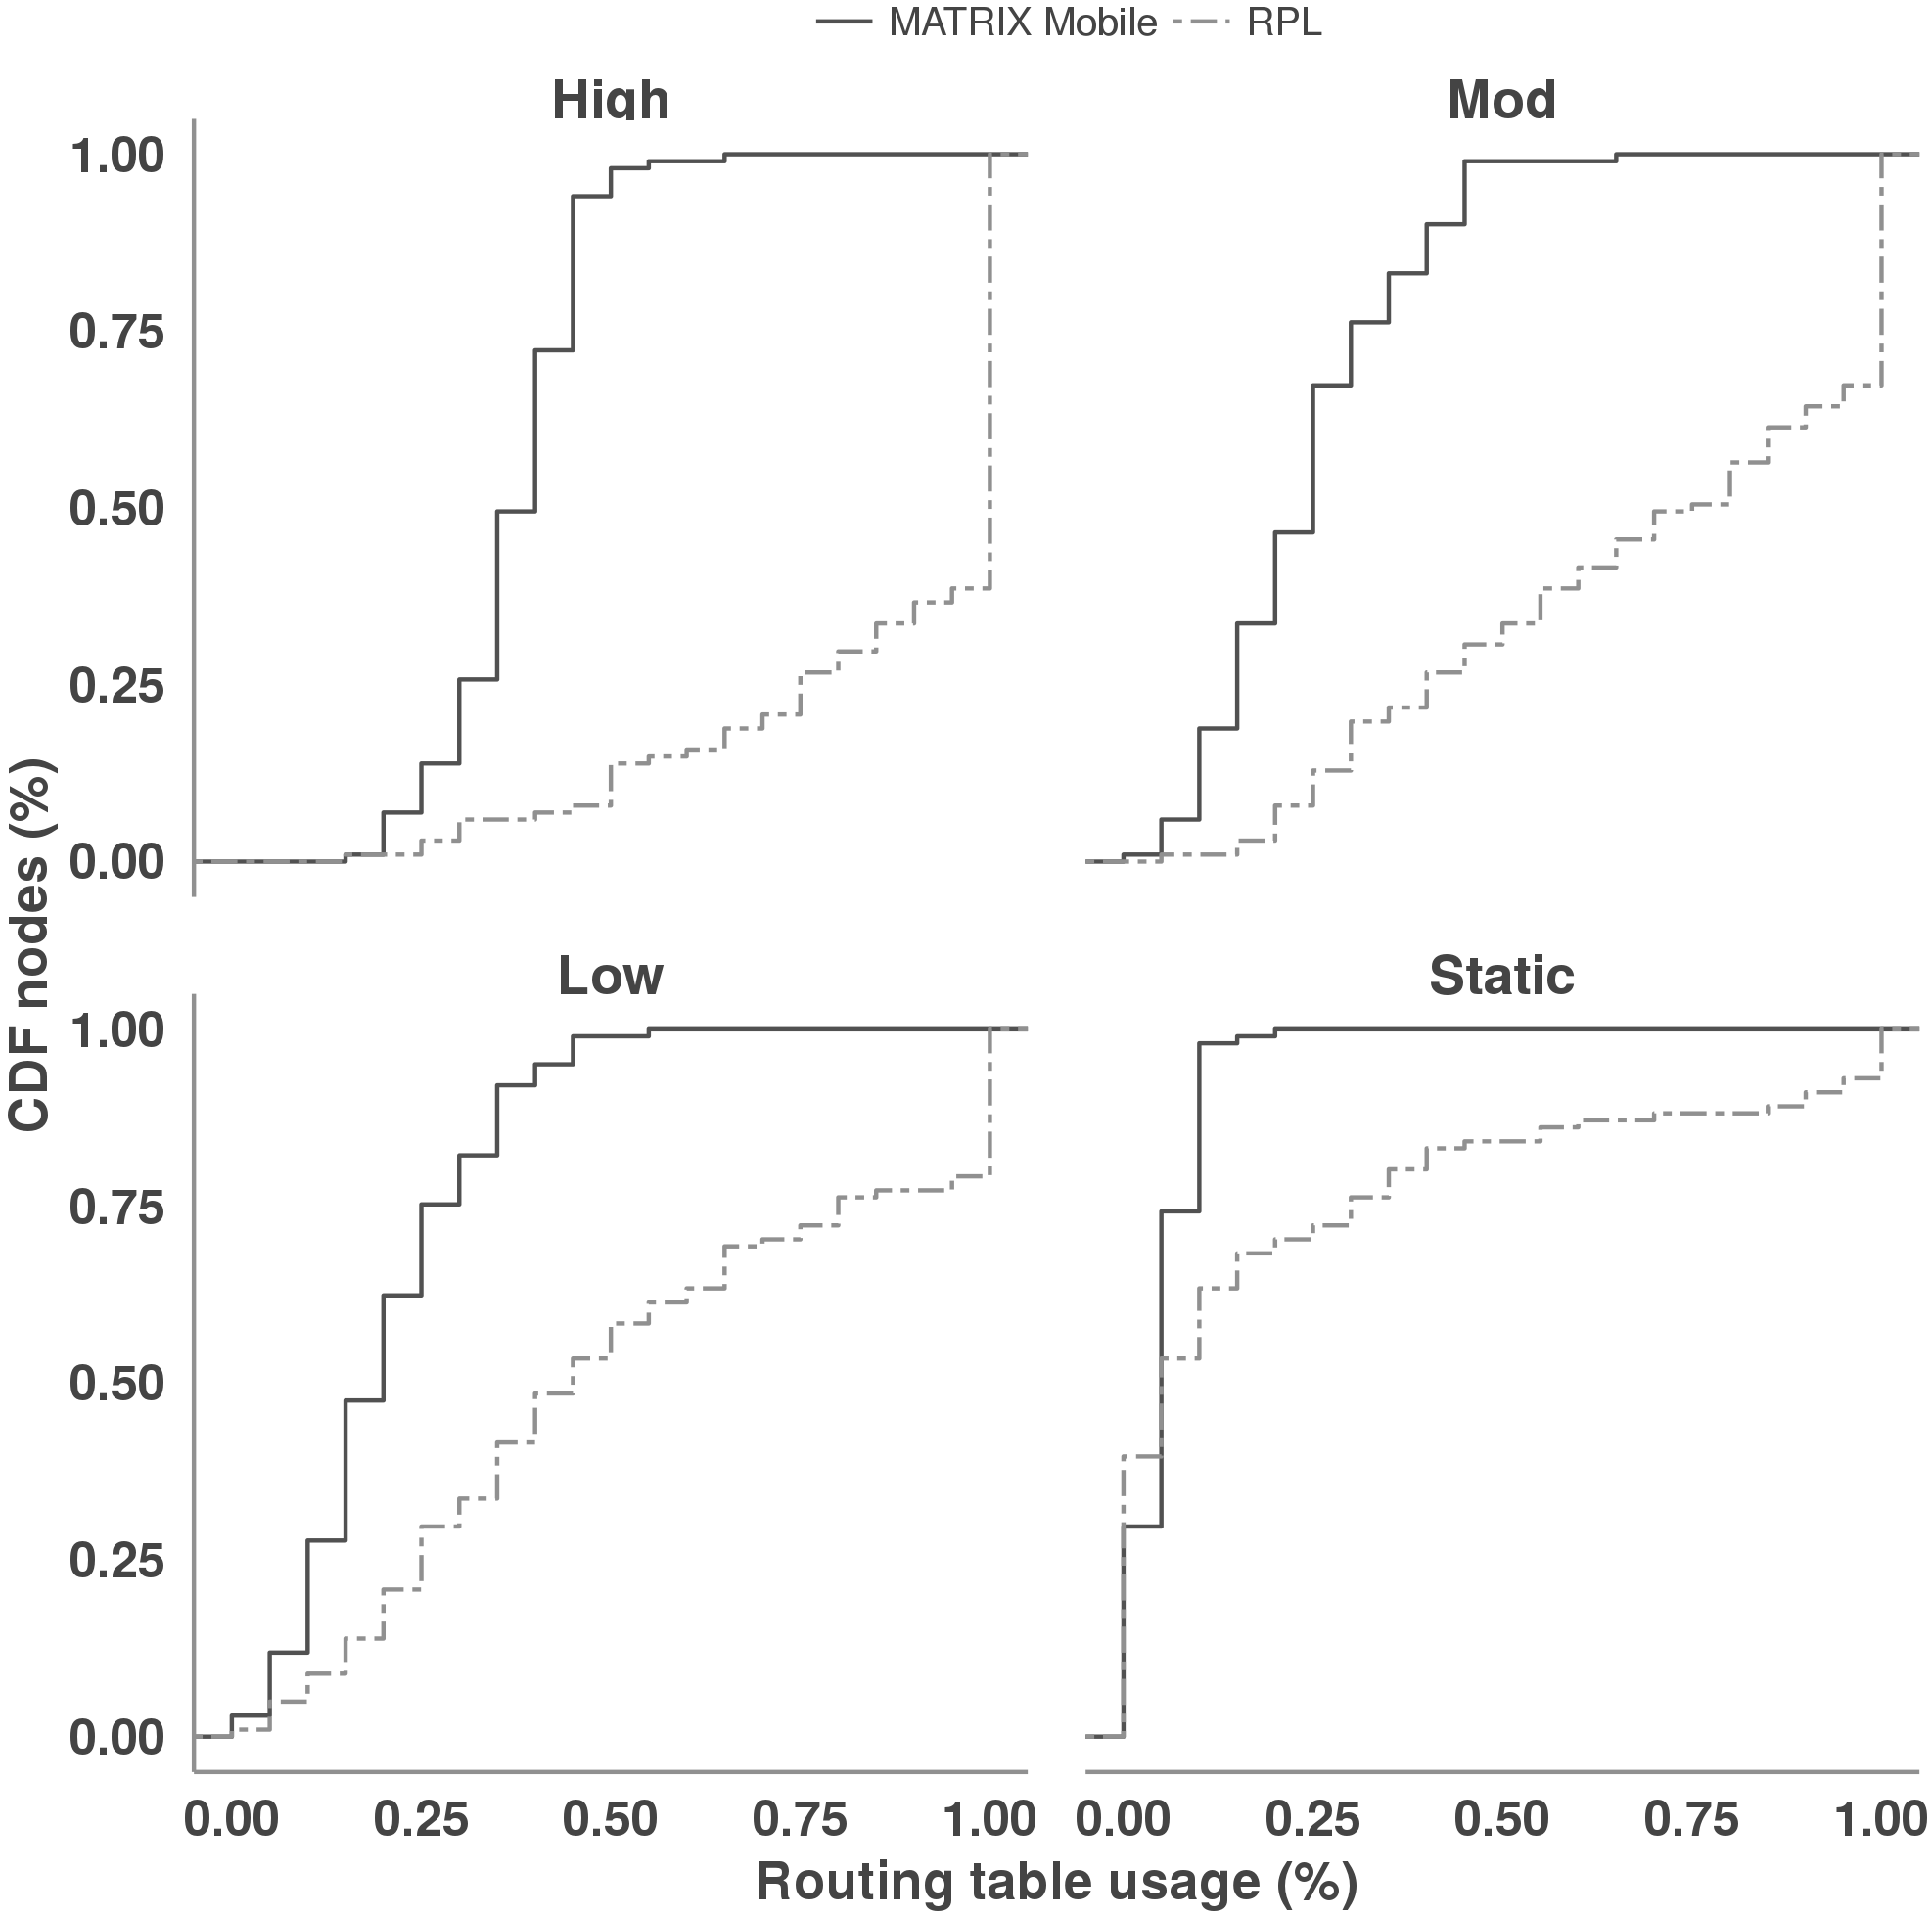
\includegraphics[width=.89\linewidth]{img/cdf-memory-grid}
\caption{CDF of routing table usage. For $\mu$Matrix $Mtable + IPchildren$, for RPL only downwards routing table. The  maximum table size is 20.}
\label{fig:memory-usage}
\end{figure}

Packets Reception Rate (PRR) is a metric of network reliability. It computes the number of packets received successfully over all packets sent. Figure~\ref{fig:prr-up} shows the PRR in bottom-up data traffic. In all scenarios, $\mu$Matrix presents higher PRR rate than RPL. When $\mu$Matrix realizes that a topological change happened, it quickly triggers the underlying route discovery, and as a consequence, bottom-up routes are rapidly rebuilt, and the reliability increases. 

Figure~\ref{fig:prr-down} shows the PRR for top-down data traffic. We can see that, when there is no mobility, $\mu$Matrix presents $99.9\%$ of success rate. In mobility scenarios, $\mu$Matrix PRR decreases slowly when more mobility is allowed. In the harshest mobility
scenario, the PRR $>75\%$. RPL, on the other hand, suffer from poor reliability, delivering $< 21.1 \%$ in all simulated scenarios, which occurs due to the lack of memory (see Figure~\ref{fig:memory-usage}) to store top-down routes.

\begin{figure*}[!t]
\begin{center}
    \subfigure[Number of control packets]
    {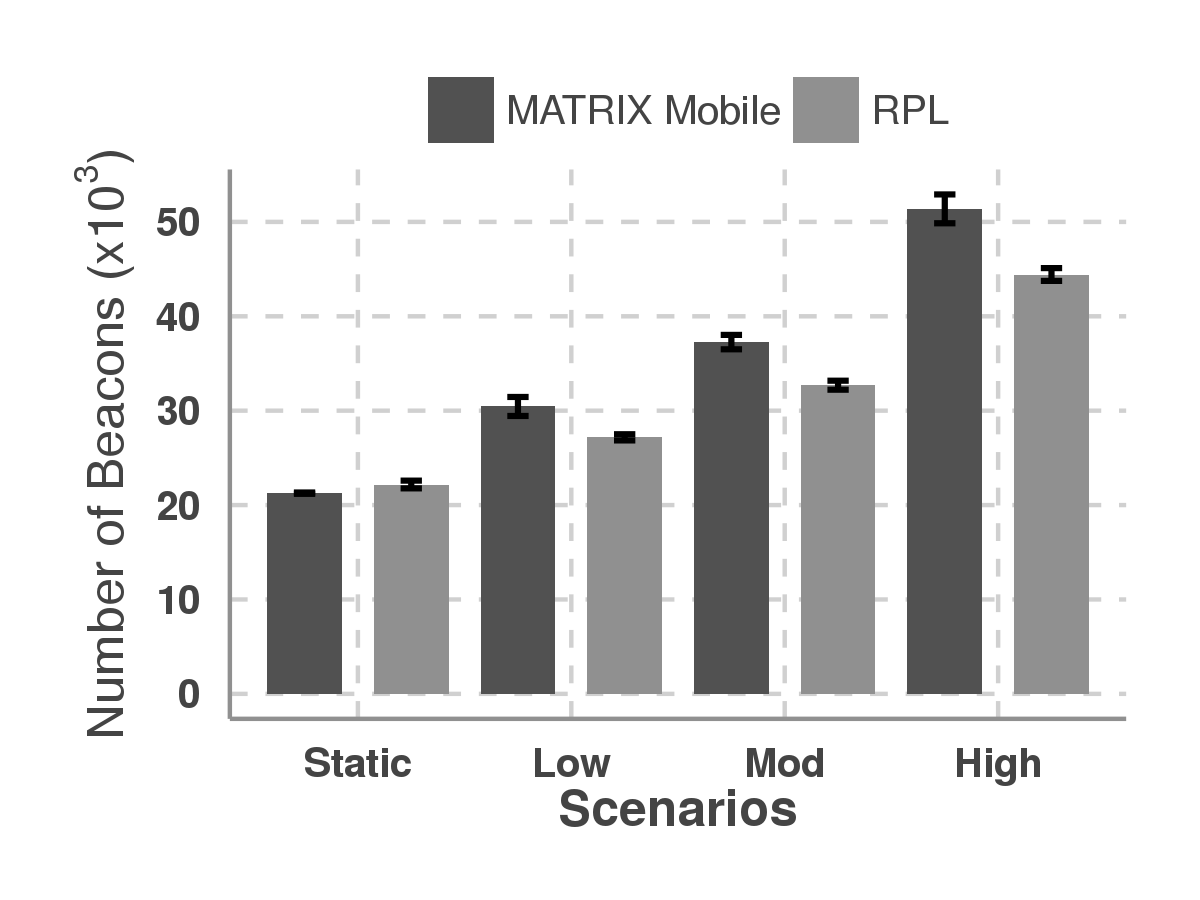
\includegraphics[width=.30\linewidth]{img/beacons}
    \label{fig:beacons}}
    \, 
    \subfigure[Bottom-up routing success rate.]
    {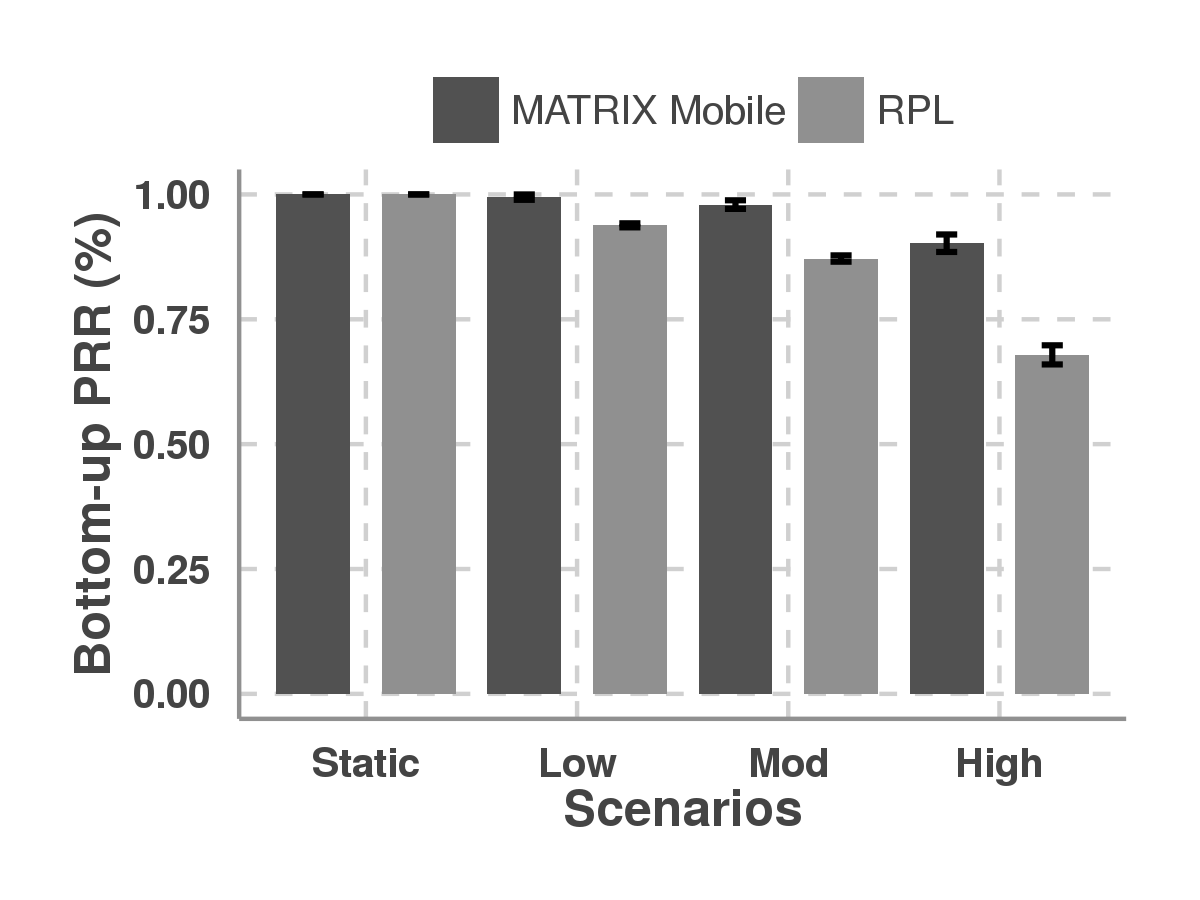
\includegraphics[width=.30\linewidth]{img/prr-up}
    \label{fig:prr-up}}
    \, 
    \subfigure[Top-down routing success rate.]
    {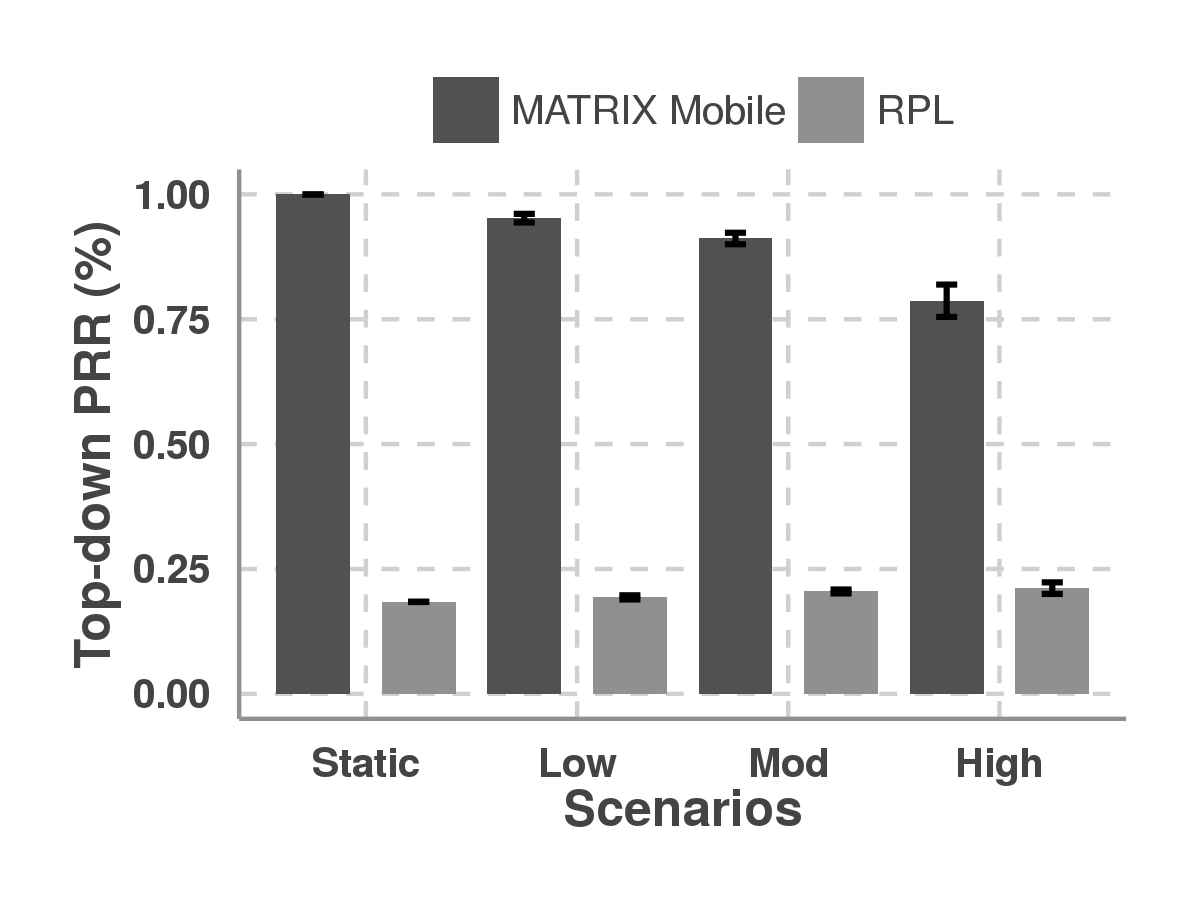
\includegraphics[width=.30\linewidth]{img/prr-down}
    \label{fig:prr-down}}
    
    \caption{Simulation experiments}
\end{center}
\end{figure*}